\section[Oscilaciones]{Oscilaciones magnéticas}
\justifying

\subsection{Conductividad longitudinal en una capa de grafeno}

\begin{frame}
  La geometría experimental consiste en una barra de Hall de grafeno
  sobre un sustrato de hBN.\\

  \begin{figure}[h]
      \centering
      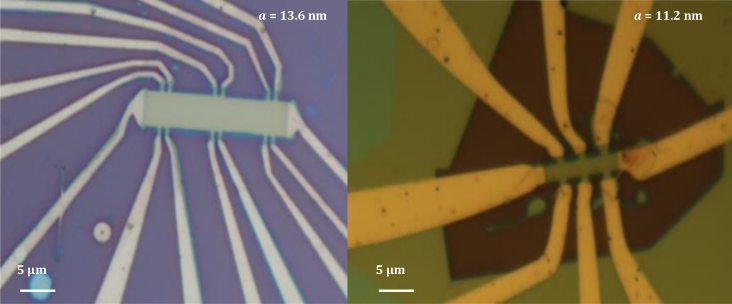
\includegraphics[scale=0.4]{graficas/hall_bar.png}
      \caption{Imágenes ópticas de barra de Hall multiterminal usadas por Kumar et Al. \cite{Kumar2017}}
      \label{Hall_bar}
  \end{figure}
\end{frame}

\begin{frame}
  Para obtener una expresión de la conductividad,
  se usará el enfoque del hamiltoniano de transferencia \cite{Illera2015}.\\
  La tasa de transición de estados se calcula usando la regla de oro de Fermi \cite{Illera2015}-\cite{Sakurai2017}:

  \begin{equation}\label{golden rule}
    d^{2}W_{l\rightarrow r \in D}=\sum_{\eta'}d^{2}W_{\eta,\eta'}=\frac{2\pi}{\hbar}\sum_{\eta'}|t_{\eta,\eta'}|^{2}\rho_{r}(\epsilon')\delta(\epsilon'-\epsilon)d\epsilon',
  \end{equation}

  $t_{\eta,\eta'}$ representa la transición entre los estados $|\eta|$ y $|\eta'|$ y $\rho(\epsilon')$ es la densidad de estados de la derecha.
\end{frame}

\begin{frame}
  La tasa de transición de los estados ocupados de la izquierda a los no ocupados de la derecha
  en el camino entre los dos contactos de la siguiente forma:
  \scriptsize
  \begin{equation}
    \Gamma_{l\rightarrow r}=\frac{2\pi}{\hbar}\sum_{\eta}\int \rho_{l}(\epsilon)f_{l}(\epsilon)\left\lbrace \int\sum_{\eta''}|t_{\eta',\eta''}|^{2}\rho_{r}(\epsilon'')[1-f_{r}(\epsilon'')]\delta(\epsilon''-\epsilon')d\epsilon''\right\rbrace d\epsilon.
  \end{equation}
  \small
  La corriente de transferencia es:
  \begin{equation}
    I=e(\Gamma_{l\rightarrow r}-\Gamma_{r\rightarrow l}).
  \end{equation}
\end{frame}

\begin{frame}
  Considerando simetria en la matriz de salto ($t_{\eta,\eta'} = t_{\eta',\eta}$),
  \begin{equation}
    I=-g\frac{2\pi e}{\hbar}\sum_{\eta'}\int |t_{\eta,\eta'}|^{2}[f(\epsilon)-f(\epsilon-eU_{g})]\textbf{Im}G_{l}^{R}(\epsilon)\mathbf{Im} G_{r}^{R}(\epsilon-eU_{g})d\epsilon,
  \end{equation}
  donde $f$, $g$ y $G_R$ son las funciones de Fermi, la degeneración y la función de Green retardada.
\end{frame}

\begin{frame}
  Los elementos de la matriz de transición se relacionan con la velocidad del electrón,
  $$v_{\eta} = \frac{1}{\hbar}\frac{\partial\zeta}{\partial k_{\eta}},$$
  mediante la relación:

  \begin{equation}
    | t_ {\eta, \eta'} |^ {2} = \frac{2 \pi \hbar^{2} }{L_{\eta} L_{\eta'}}v_{\eta} v_{\eta'}.
  \end{equation}
\end{frame}

\begin{frame}
  La conductividad se obtiene de la siguiente manera:
  \begin{equation}
    \sigma_{xx} = \frac{L_x}{L_y}\left(\frac{dI}{dU_g}\right)_{U_g=0},
  \end{equation}

  \begin{equation}
    \sigma_{xx}=\sigma_{o}\sum_{n,k_{y},\beta}\int |t_{x,x}|^{2}\left(-\frac{\partial f}{\partial\epsilon'}\right)\left[2\textbf{Im}G_{n,k}^{R}(\epsilon')\right]^{2}d\epsilon,
    \label{eq:conductividad}
  \end{equation}

  donde se ha tomado $\rho(\epsilon) = - \frac{1}{\pi}\textbf{Im} G_{R} (\epsilon)$,
  $\sigma_{o} = \frac{2 e^{2} n_{L} L_{x}}{\pi \hbar L_{y}}$,
  $ L_{x (y)} $ son las dimensiones de la muestra y $ n_{L} = \Phi / \Phi_{o} $, ($\Phi_{0} = \frac{2\pi}{\hbar})$.
\end{frame}

\subsection{Oscilaciones magnéticas a altas temperaturas}

\begin{frame}
  A partir de la ecuación \ref{eq:conductividad}, se toma:

  \begin{equation}
    [2\textbf{Im}G^{R}(\epsilon)]^2 = G_{R}^{2}+G_{A}^{2}-2G_{R}G_{A},
    \label{2ImGr2}
  \end{equation}
  $G_A$ es la función avanzada de Green que toma la forma \cite{Vega2016}-\cite{Salazar2016}:
  \begin{equation}
    G_A(\epsilon) = \frac{1}{\epsilon'-\epsilon_n-\Sigma^A(\epsilon)} + \frac{1}{\epsilon'+\epsilon_n-\Sigma^A(\epsilon)},
   \end{equation}
\end{frame}

\begin{frame}
\end{frame}

\begin{frame}
\end{frame}

\begin{frame}
\end{frame}

\begin{frame}
\end{frame}

\subsection{Tiempo de relajación del electrón}

\begin{frame}
\end{frame}

\begin{frame}
\end{frame}

\begin{frame}
\end{frame}

\begin{frame}
\end{frame}

\begin{frame}
\end{frame}
